\documentclass[11pt]{article}
\usepackage{graphicx}
\usepackage{hyperref}
\usepackage{natbib}
\usepackage{amsmath}
\usepackage{enumitem}
\usepackage{mathtools}

\setlength{\textwidth}{6.5in}
\setlength{\headheight}{0in}
\setlength{\textheight}{8.0in}
\setlength{\hoffset}{0in}
\setlength{\voffset}{0in}
\setlength{\oddsidemargin}{0in}
\setlength{\evensidemargin}{0in}

\title{PS7}
  
\author{Shihong Pan\\ \url{https://github.com/PSH-hub24/phys-ga2000}}


\begin{document}

\maketitle

\section*{Q1}
\begin{enumerate}[label=(\alph*)]
    \item The gravitational force exerted on the Moon by the Earth is
    \begin{equation}
        F_{\text{moon}}=\frac{GMm}{R^2}\coloneqq m\omega^2R
    \end{equation}
    so $\omega$ can be written as $\omega^2=GM/R^3$. Now, the satellite has the same angular frequency at L1, so the centripetal force it experiences is
    \begin{equation}
        F_{\text{sate}}=m\omega^2r.
    \end{equation}
    The field strength at the satellite is the sum of the field strength due to the Earth and the Moon
    \begin{equation}
        g_{\text{sate}} = \frac{GM}{r^2}-\frac{Gm}{(R-r)^2}=\frac{F_{\text{sate}}}{m}=\omega^2r=\frac{GMr}{R^3}.
    \end{equation}
    To rescale the equation, substitute $m=m'M$ and $r=r'R$ into the equation above, such that
    \begin{equation}
        \frac{GM}{r'^2R^2}-\frac{Gm'M}{R^2(1-r')^2}=\frac{GMr'R}{R^3}.
    \end{equation}
    Multiply $R^2/M$ on both sides and rearrange to get
    \begin{equation}
        f(r')=\frac{G}{r'^2}-\frac{Gm'}{(1-r')^2}-Gr'=0.
    \end{equation}
    where $m'$ is a constant depending on the masses of the two planets. 
    
    \item The codes compute the root of $f(r')$ by first using a simple bracketing function to find an interval that includes a root, and use the mid-point of the interval as the initial guess for Newton's method (please see the codes for details). The derivative of $f(r')$ is obtained by using jax.grad.

    Fig \ref{fig:Q1} shows the initial guesses and the $r'$ values for all three cases (the Earth and the Moon, the Earth and the Sun, the Jupiter-mass planet and the Sun). Note that in the later two cases, $r'$ measures the relative distance from the Sun to the other planet. So if we want to talk about the distance $r$ from the Earth in all three cases, we have
    \begin{itemize}
        \item The Earth and the Moon: $r'\approx0.8489$, $R=3.844\times 10^5$ km, so $r=3.263\times 10^5$ km.
        \item The Earth and the Sun: $r'\approx1-0.9900=0.0100$, $R=1.49\times 10^8$ km, so $r=1.49\times 10^6$ km.
        \item The Jupiter-mass planet and the Sun: $r'\approx1-0.9333=0.0667$, $R=3.844\times 10^5$ km, so $r=2.5639\times 10^4$ km.
    \end{itemize}
\end{enumerate}

\section*{Q2}
For the parabolic approximation I used the one given in the root-finding lecture notes (section 4 Brent's method). Then I just followed the description given in the minimization lecture notes (section 4 Brent's 1d minimization). I set the termination condition by comparing the change between the previous minimum value and the current minimum value to the magnitude of the current minimum value times a tolerance (I set the tolerance to 1e-15). If the change is smaller than the tolerance, then the iterations terminate. Fig \ref{fig:Q2} shows the output of my Brent function and that of scipy.optimize.brent. It turns out that my number is closer to 0.3.

\begin{figure}[b!]
\centering
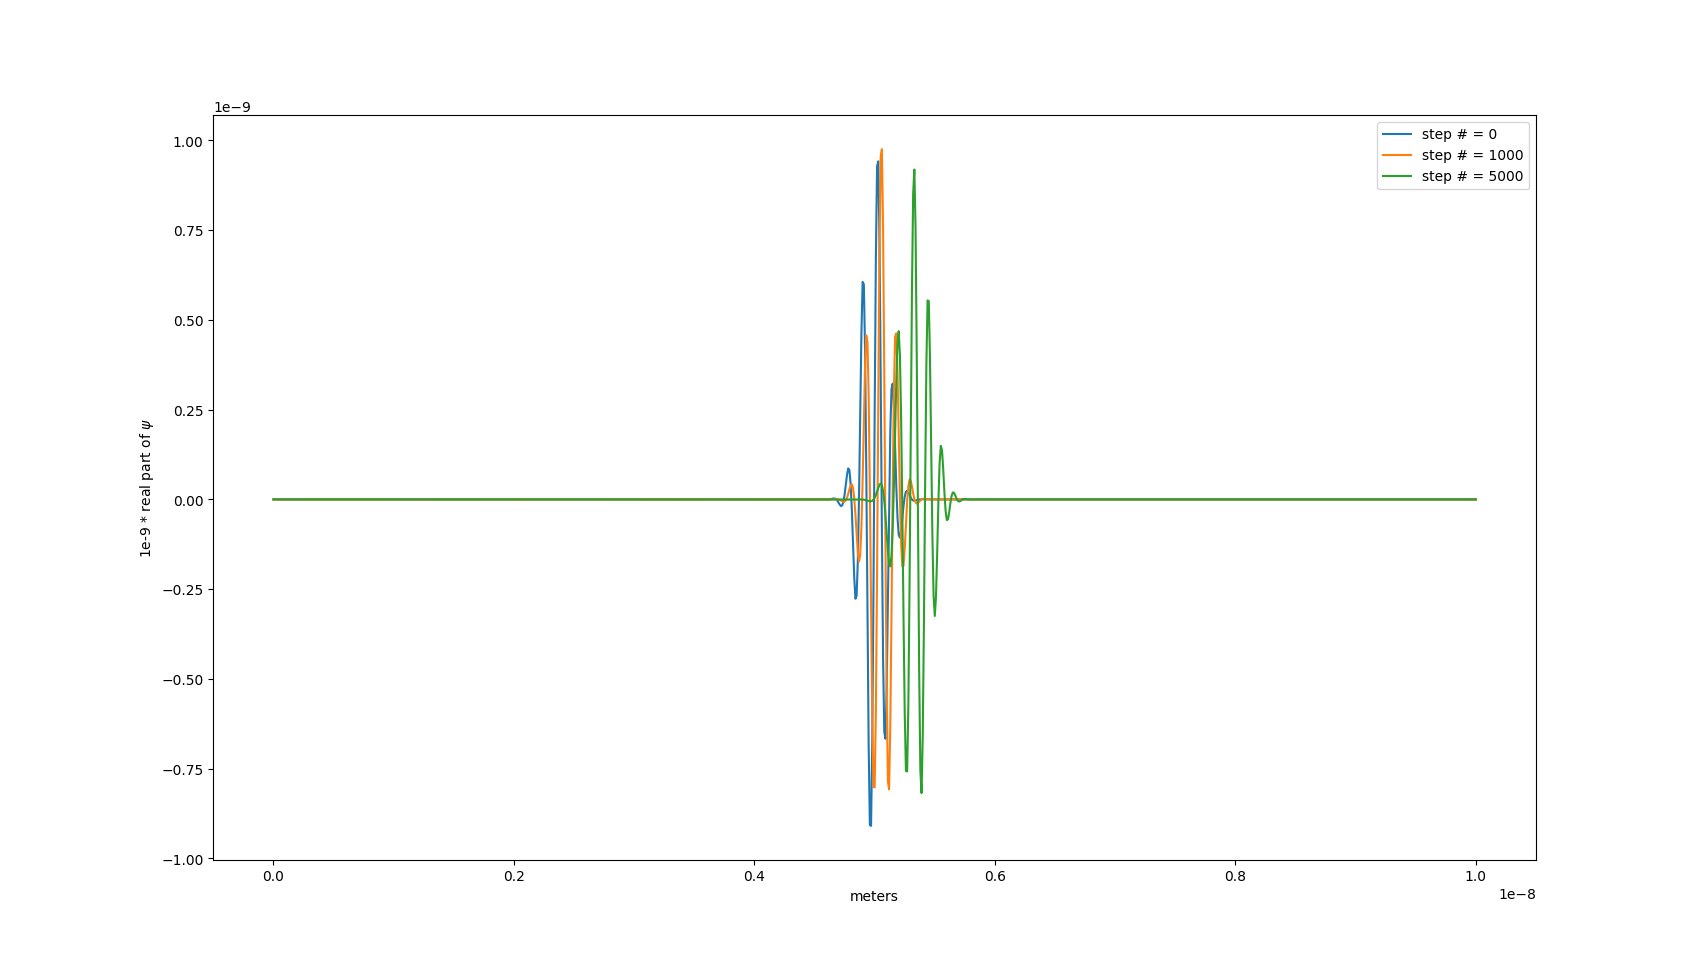
\includegraphics[width=1\textwidth]{Computational Physics/ps7Figures/q1.png}
\caption{The $r/R$ values and the initial guesses.}
  \label{fig:Q1}
\end{figure}

\begin{figure}[b!]
\centering
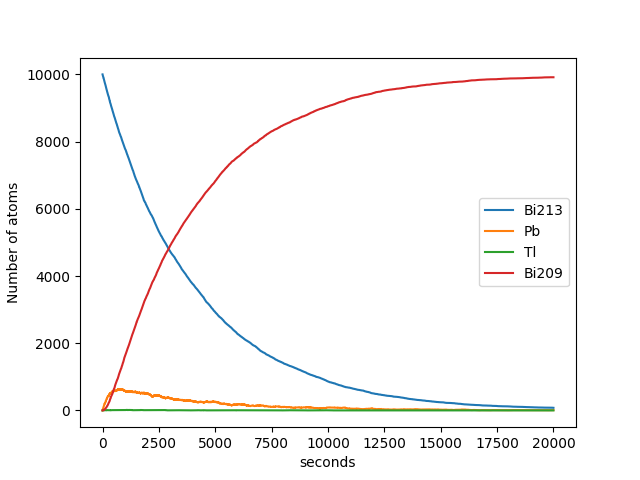
\includegraphics[width=1\textwidth]{Computational Physics/ps7Figures/q2.png}
\caption{Compare my Brent's 1d minimization to scipy's minimization.}
  \label{fig:Q2}
\end{figure}


\bibliographystyle{apj}
\bibliography{example}

\end{document}

 
 
